%!TEX program = pdflatex
\documentclass{elegantpaper}

\title{ElegantPaper: An Elegant \LaTeX{} Template for Working Paper}
\author{\href{https://ddswhu.me/}{Dongsheng Deng} %
		\thanks{Thank Peiyi Yao for good suggestions.} \\[0.5ex] %
		Elegant\LaTeX{} Group}
\date{\small\itshape Version: 0.01 \\ Last update: \today}

\begin{document}

\maketitle

\begin{abstract}
	This paper illustrates the usage of the ElegantPaper template, which is designed for writing working paper. This template is based on the standard \LaTeX{} article class. The goal of this template is to make the writing process easier and more comfortable. You can get rid of all the worries about format. Just enjoy it, if you have any questions or suggestions, please contact me at: \email{ddswhu@outlook.com}.
\end{abstract}

\section{Introduction}

This template is based on the standard \LaTeX{} article class, which means you can pass the arguments of article class to it (\verb|a4paper|, \verb|12pt| and etc.).

\subsection{Font Settings}
I change the default article font computer modern to \verb|newtx| series, and the default font size is set to \verb|11pt|.

\begin{itemize}[noitemsep]
	\item \verb|newtxtext| package for text font, similar to times new roman font.
	\item \verb|newtxmath| package for math font, close to \verb|times| and \verb|mtpro2| packages.
	\item \verb|newtxtt| package for typewriter font, with option \verb|scale = 0.8|.
\end{itemize}

These packages operate perfectly but are inappropriate for big operators, for example \verb|\sum| and \verb|\prod|, thus, I change these operators back to computer modern font. Equation~\eqref{eq:binom} shows the effects of these fonts:
\begin{equation}
(a+b)^{n} = \sum_{k=0}^{n} C_{n}^{k} a^{n-k} b^k \label{eq:binom}
\end{equation}



The \verb|\linespread| (controls line spacing) is set to 1.3, and I use \verb|microtype| to improve the font justification. \verb|type1cm| package is used to remove the font shape and font size warning messages.

\subsection{Custom Commands}

I don't change any default command or environment, which means you can use all the basic \LaTeX{} commands and environments as before.  Besides, I define 3 commands
\begin{enumerate}[noitemsep]
	\item \verb|\email{#1}|: create the hyperlink to email address.
	\item \verb|\figref{#1}|: same usage as \verb|\ref{#1}|, but start with label text <\textbf{Figure n}>.
	\item \verb|\tabref{#1}|: same usage as \verb|\ref{#1}|, but start with label text <\textbf{Table n}>.
\end{enumerate}{}

\subsection{List Environments}
When you are using \verb|itemize|, \verb|enumerate|, or \verb|description| environment, please add the \verb|noitemsep| option to these environments. For example, \\

\begin{minipage}[c]{0.45\linewidth}
\begin{Verbatim}[tabsize=4,frame=single,baselinestretch=1]
\begin{itemize}[noitemsep]
	\item Routing and resource discovery;
	\item Resilient and scalable networks;
	\item Distributed storage and search.
\end{itemize}
\end{Verbatim}
\end{minipage}
\begin{minipage}[c]{0.45\linewidth}
\begin{itemize}[noitemsep]
	\item Routing and resource discovery;
	\item Resilient and scalable computer networks;
	\item Distributed storage and search.
\end{itemize}
\end{minipage}

\subsection{Table}
I strongly recommend you to use the \verb|booktabs| package in your paper. It adds three commands to make the table prettier, ie. \verb|\toprule|, \verb|\midrule| and \verb|\bottomrule|. Here is an example.

\begin{table}[!htbp]
  \small
  \centering
  \caption{Regression Result Example}
    \begin{tabular}{lll}
    \toprule
          & \multicolumn{1}{c}{(1)} & \multicolumn{1}{c}{(2)} \\
      & \multicolumn{1}{c}{price} & \multicolumn{1}{c}{price} \\
    \midrule
    mpg   & \multicolumn{1}{c}{-238.9***} & \multicolumn{1}{c}{-49.51} \\
          & \multicolumn{1}{c}{(53.08)} & \multicolumn{1}{c}{(86.16)} \\
    weight & \multicolumn{1}{c}{} & \multicolumn{1}{c}{1.747***} \\
          & \multicolumn{1}{c}{} & \multicolumn{1}{c}{(0.641)} \\
    constant & \multicolumn{1}{c}{11,253***} & \multicolumn{1}{c}{1,946} \\
          & \multicolumn{1}{c}{(1,171)} & \multicolumn{1}{c}{(3,597)} \\
    observations & \multicolumn{1}{c}{74} & \multicolumn{1}{c}{74} \\
    R-squared & \multicolumn{1}{c}{0.220} & \multicolumn{1}{c}{0.293} \\
    \midrule
    \multicolumn{3}{l}{\scriptsize Standard errors in parentheses} \\
    \multicolumn{3}{l}{\scriptsize *** p<0.01, ** p<0.05, * p<0.1} \\
    \end{tabular}%
  \label{tab:reg}%
\end{table}%



\subsection{Graphics}
To include a graphic, you can use figure environment as usual. \figref{fig:mpg} shows the effect. You can put all your images in the sub directories (\verb|./image/|, \verb|./img/|, \verb|./figure/|, \verb|./fig/|) of your current working directory.

\begin{Verbatim}[tabsize=4,frame=single,baselinestretch=1]
\begin{figure}[!ht]
	\centering
	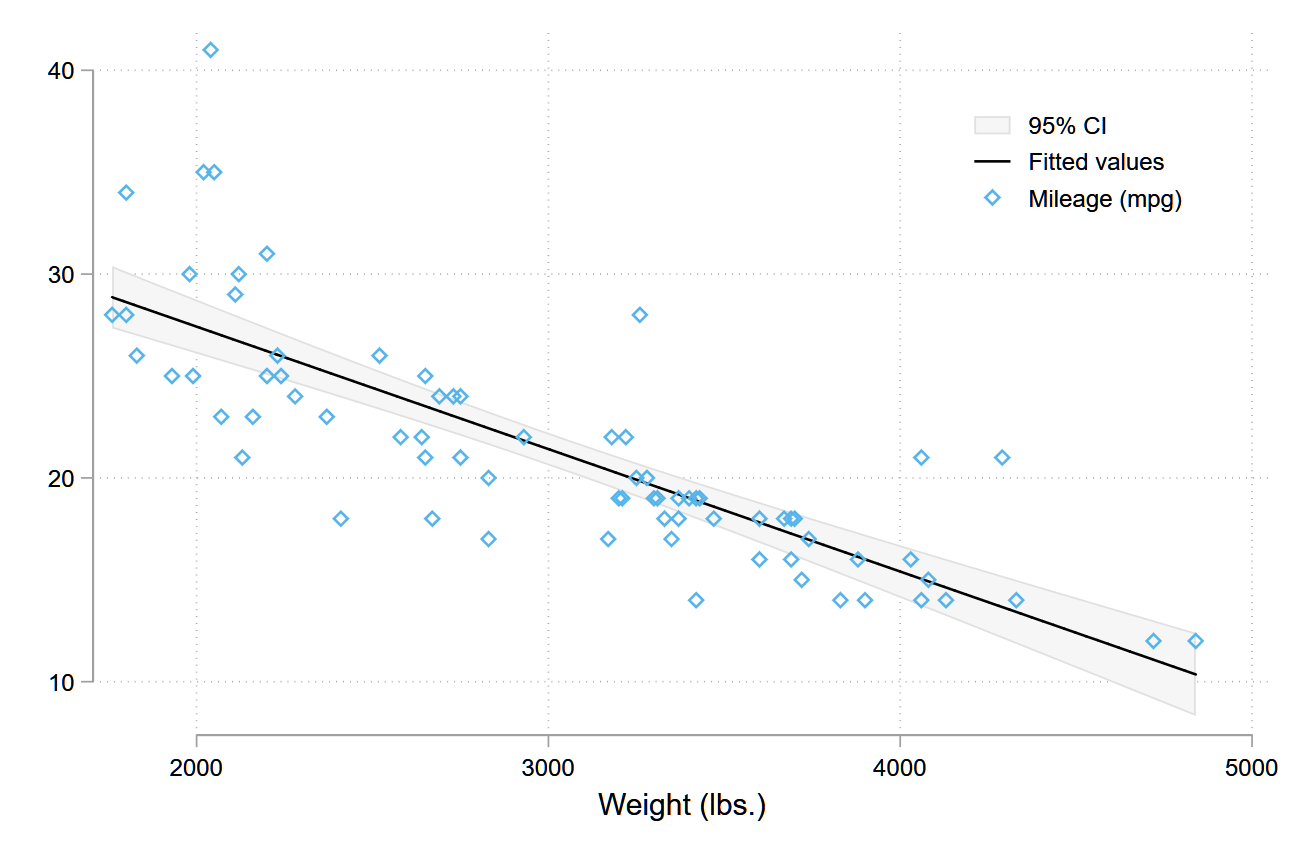
\includegraphics[width=0.6\textwidth]{mpg.png}
	\caption{The Relationship between MPG and Weight\label{fig:mpg}}
\end{figure}
\end{Verbatim}
\begin{figure}[!ht]
	\centering
	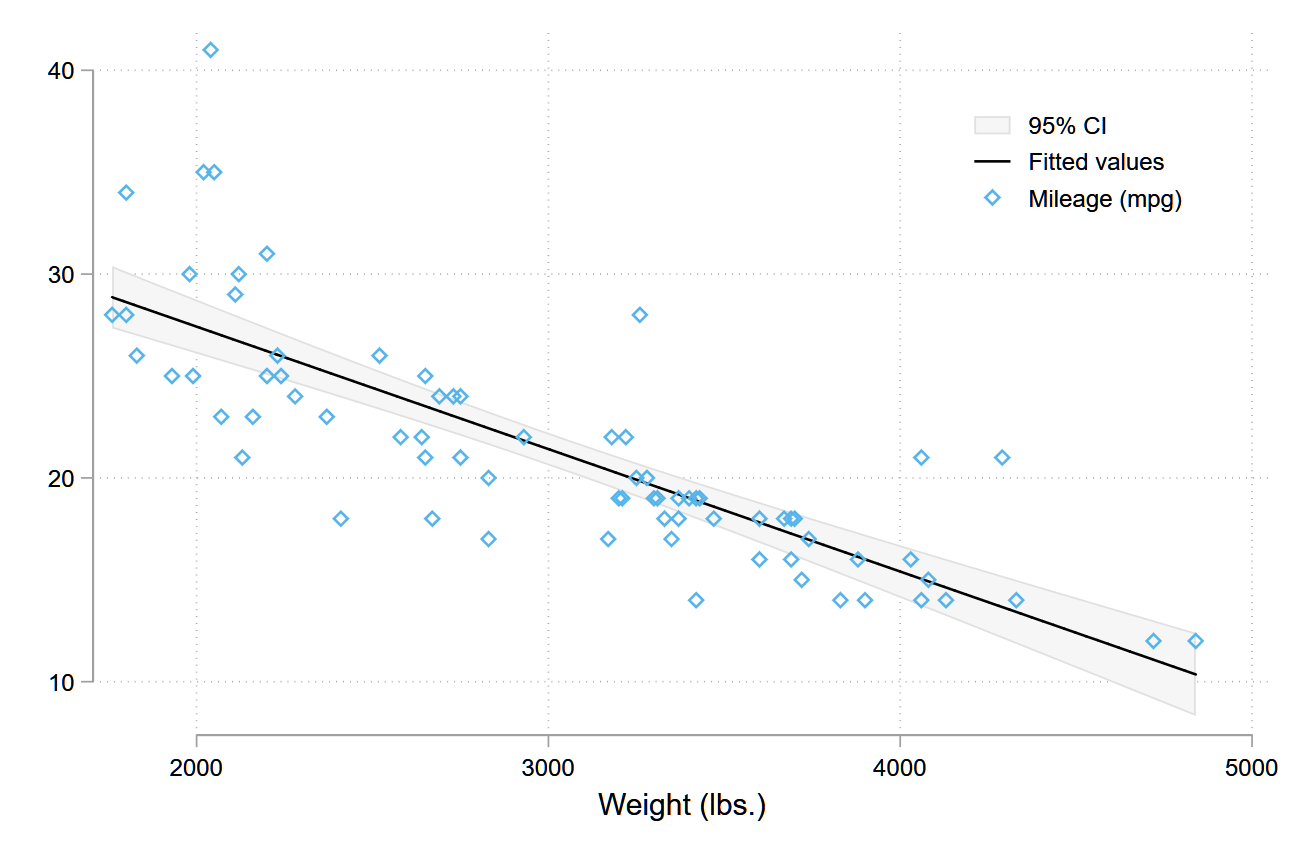
\includegraphics[width=0.6\textwidth]{mpg.png}
	\caption{The Relationship between MPG and Weight\label{fig:mpg}}
\end{figure}

\subsection{Bibliography}
This template uses Bib\TeX{} to generate the bibliography, the default bibliography style is \verb|aer|. ~\cite{Chen2018} use data from a major peer-to-peer lending marketplace in China to study whether female and male investors evaluate loan performance differently. You can add bib items (from Google Scholar, Mendeley, EndNote, and etc.) to \verb|wp_ref.bib| file, and cite the bibkey in the \verb|tex| file.


\nocite{EINAV2010,Havrylchyk2018} 

\bibliographystyle{aer}
\bibliography{wp_ref}
\end{document}
